\documentclass[aspectratio=169]{beamer}
% Add slides directory to search path for Dartmouth theme
\makeatletter
\def\input@path{{../}}
\makeatother
\usetheme{Dartmouth}
\usepackage{booktabs}
\usepackage{listings}
\usepackage{tikz}
\usetikzlibrary{arrows.meta,positioning,shapes,decorations.pathreplacing}
\usepackage{hyperref}
\usepackage{xcolor}
\usepackage{graphicx}
\usepackage{fontspec}
\usepackage{tcolorbox}
\usepackage{amsmath}
\usepackage{amssymb}

% Color scheme
\definecolor{darkblue}{RGB}{0,82,155}
\definecolor{lightblue}{RGB}{100,181,246}
\definecolor{darkgreen}{RGB}{46,125,50}
\definecolor{orange}{RGB}{255,152,0}
\definecolor{purple}{RGB}{142,36,170}
\definecolor{thinkbox}{RGB}{255,245,220}
\definecolor{discussbox}{RGB}{230,240,255}

\setbeamercolor{frametitle}{bg=darkblue}
\setbeamercolor{progress bar}{fg=lightblue,bg=lightblue!30}

% Code listing settings
\lstset{
    basicstyle=\ttfamily\small,
    breaklines=true,
    frame=single,
    backgroundcolor=\color{gray!10},
    keywordstyle=\color{darkblue}\bfseries,
    commentstyle=\color{darkgreen}\itshape,
    stringstyle=\color{orange},
    showstringspaces=false,
    language=Python
}

% Custom boxes
\newtcolorbox{thinkaboutit}{
    colback=thinkbox,
    colframe=orange,
    title=💭 Think about it!,
    fonttitle=\bfseries
}

\newtcolorbox{discussion}{
    colback=discussbox,
    colframe=blue,
    title=💬 Discussion,
    fonttitle=\bfseries
}

\title{Lecture 18: GPT Architecture}
\subtitle{Generative Pre-Training for Language 🤖}
\author{Models of Language and Conversation}
\institute{Dr. Jeremy R. Manning}
\date{Week 7}

\begin{document}

% Title slide
\begin{frame}
    \titlepage
\end{frame}

% Table of contents
\begin{frame}{Today's Journey 🗺️}
    \tableofcontents
\end{frame}

\section{Introduction to GPT}

\begin{frame}{The GPT Revolution 🚀}
    \begin{discussion}
        What made GPT different from previous language models?
    \end{discussion}

    \vspace{0.3cm}

    \textbf{Key Innovation: Pre-training + Fine-tuning}
    \begin{itemize}\setlength{\itemsep}{0pt}
        \item 📚 \textbf{Pre-train} on massive unlabeled text (unsupervised)
        \item 🎯 \textbf{Fine-tune} on specific tasks (supervised)
        \item 🔄 Transfer learning for NLP
        \item 🎨 One model, many tasks
    \end{itemize}

    \vspace{0.3cm}

    \begin{alertblock}{Paradigm Shift}
        Before GPT: Task-specific models trained from scratch \\
        After GPT: General-purpose models adapted to tasks
    \end{alertblock}

    \vspace{0.3cm}

    \small
    \textit{Reference: Radford et al. (2018) - "Improving Language Understanding by Generative Pre-Training"}
\end{frame}

\begin{frame}[shrink=10]{From BERT to GPT: Different Approaches 🔀}
\small
    \begin{columns}[T]
        \begin{column}{0.48\textwidth}
            \textbf{BERT (2018):}
            \begin{itemize}\setlength{\itemsep}{0pt}
                \item 🎭 \textbf{Masked Language Model}
                \item Bidirectional context
                \item Fill in the blank
                \item Great for understanding
                \item Not designed for generation
            \end{itemize}

            \vspace{0.15cm}

            \textit{Example:}
            "The [MASK] sat on the mat"
        \end{column}

        \begin{column}{0.48\textwidth}
            \textbf{GPT (2018):}
            \begin{itemize}\setlength{\itemsep}{0pt}
                \item ➡️ \textbf{Autoregressive Model}
                \item Left-to-right (causal)
                \item Predict next token
                \item Natural for generation
                \item Can also understand
            \end{itemize}

            \vspace{0.15cm}

            \textit{Example:}
            "The cat sat" → predict "on"
        \end{column}
    \end{columns}

    \vspace{0.3cm}

    \begin{thinkaboutit}
        Why is autoregressive modeling more natural for text generation?
    \end{thinkaboutit}
\end{frame}

\begin{frame}[shrink=5]{The Transformer Decoder 🏗️}
    \textbf{GPT uses the Transformer \textit{decoder} architecture}

    \vspace{0.3cm}

    \begin{center}
        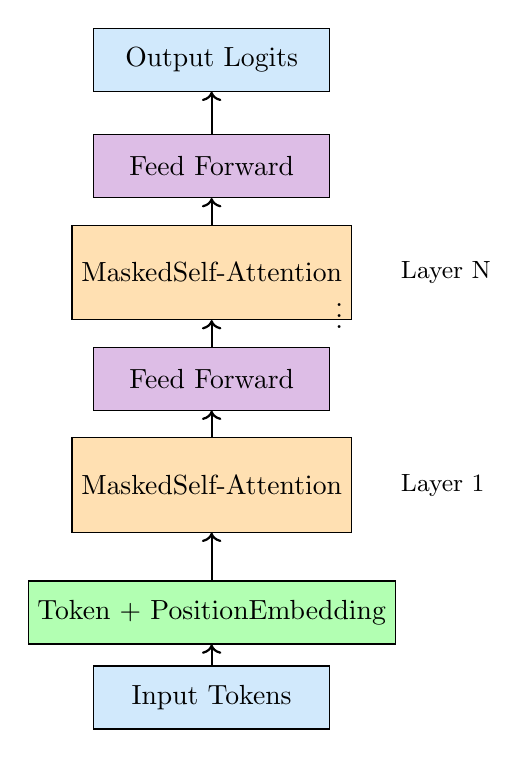
\begin{tikzpicture}[scale=0.9]
            % Input
            \node[draw, rectangle, fill=lightblue!30, minimum width=3cm, minimum height=0.8cm] (input) at (0,0) {Input Tokens};

            % Embedding
            \node[draw, rectangle, fill=green!30, minimum width=3cm, minimum height=0.8cm] (embed) at (0,1.2) {Token + Position\\Embedding};

            % Decoder blocks
            \node[draw, rectangle, fill=orange!30, minimum width=3cm, minimum height=1.2cm] (dec1) at (0,3) {Masked\\Self-Attention};
            \node[draw, rectangle, fill=purple!30, minimum width=3cm, minimum height=0.8cm] (ffn1) at (0,4.5) {Feed Forward};

            \node[draw, rectangle, fill=orange!30, minimum width=3cm, minimum height=1.2cm] (dec2) at (0,6) {Masked\\Self-Attention};
            \node[draw, rectangle, fill=purple!30, minimum width=3cm, minimum height=0.8cm] (ffn2) at (0,7.5) {Feed Forward};

            % Output
            \node[draw, rectangle, fill=lightblue!30, minimum width=3cm, minimum height=0.8cm] (output) at (0,9) {Output Logits};

            % Arrows
            \draw[->, thick] (input) -- (embed);
            \draw[->, thick] (embed) -- (dec1);
            \draw[->, thick] (dec1) -- (ffn1);
            \draw[->, thick] (ffn1) -- (dec2);
            \draw[->, thick] (dec2) -- (ffn2);
            \draw[->, thick] (ffn2) -- (output);

            % Labels
            \node[right=0.5cm of dec1] {\small Layer 1};
            \node[right=0.5cm of dec2] {\small Layer N};
            \node at (1.8, 5.5) {$\vdots$};
        \end{tikzpicture}
    \end{center}

    \vspace{0.3cm}

    \textbf{Key: Masked attention prevents "peeking" at future tokens!}
\end{frame}

\section{GPT Architecture Details}

\begin{frame}[shrink=5]{Masked Self-Attention 👀}
    \textbf{The Core Innovation: Causal Masking}

    \vspace{0.3cm}

    \begin{center}
        \begin{tikzpicture}[scale=0.7]
            % Attention matrix
            \foreach \i in {1,...,5} {
                \foreach \j in {1,...,5} {
                    \pgfmathparse{\j <= \i ? 30 : 0}
                    \edef\opacity{\pgfmathresult}
                    \fill[blue!\opacity] (\j*1.2, -\i*1.2) rectangle +(1, 1);
                    \draw (\j*1.2, -\i*1.2) rectangle +(1, 1);
                }
            }

            % Labels
            \node at (0.5, 0.5) {\small Tokens};
            \foreach \i in {1,...,5} {
                \node at (\i*1.2 + 0.5, 0.3) {\small $t_\i$};
                \node at (0, -\i*1.2 + 0.5) {\small $t_\i$};
            }

            % Legend
            \node[right] at (7, -2) {\textcolor{blue!30}{■} Can attend};
            \node[right] at (7, -3) {□ Masked (cannot attend)};
        \end{tikzpicture}
    \end{center}

    \vspace{0.3cm}

    \textbf{Each token can only attend to itself and previous tokens}
    \begin{itemize}\setlength{\itemsep}{0pt}
        \item Ensures autoregressive property
        \item No information leakage from future
        \item Allows parallel training
    \end{itemize}
\end{frame}

\begin{frame}[shrink=10]{Position Encoding in GPT 📍}
    \textbf{Why we need position information:}

    \vspace{0.3cm}

    \begin{block}{The Problem}
        Self-attention is \textit{permutation invariant}—it doesn't inherently know word order!
    \end{block}

    \vspace{0.3cm}

    \textbf{GPT's Solution: Learned Position Embeddings}
    \begin{itemize}\setlength{\itemsep}{0pt}
        \item Each position gets a learnable embedding
        \item Added to token embeddings: $x_i = \text{token}_i + \text{pos}_i$
        \item Model learns position patterns during training
        \item Maximum sequence length: 512 tokens (GPT-1)
    \end{itemize}

    \vspace{0.3cm}

    \begin{columns}[T]
        \begin{column}{0.5\textwidth}
            \textbf{Alternative: Sinusoidal} \\
            \small (Used in original Transformer)
            \begin{itemize}\setlength{\itemsep}{0pt}
                \item Fixed function
                \item Generalizes to longer sequences
            \end{itemize}
        \end{column}
        \begin{column}{0.5\textwidth}
            \textbf{GPT: Learned} \\
            \small (More flexible)
            \begin{itemize}\setlength{\itemsep}{0pt}
                \item Learned from data
                \item Task-specific patterns
            \end{itemize}
        \end{column}
    \end{columns}
\end{frame}

\begin{frame}{GPT-1 Model Specifications 📊}
    \begin{table}
        \begin{tabular}{ll}
            \toprule
            \textbf{Component} & \textbf{Value} \\
            \midrule
            Parameters & 117M \\
            Layers & 12 \\
            Hidden size & 768 \\
            Attention heads & 12 \\
            Max sequence length & 512 tokens \\
            Vocabulary size & 40,000 (BPE) \\
            Training data & BooksCorpus (7,000 books) \\
            Training tokens & ~5 billion \\
            \bottomrule
        \end{tabular}
    \end{table}

    \vspace{0.3cm}

    \textbf{Training objective:}
    $$\mathcal{L} = \sum_{i} \log P(t_i | t_{<i}; \Theta)$$

    Maximize likelihood of next token given previous context
\end{frame}

\begin{frame}[fragile]{GPT Architecture in Code 💻}
\begin{lstlisting}[language=Python]
import torch.nn as nn

class GPTBlock(nn.Module):
    def __init__(self, d_model, n_heads):
        super().__init__()
        self.attention = MaskedMultiHeadAttention(d_model, n_heads)
        self.norm1 = nn.LayerNorm(d_model)
        self.ffn = nn.Sequential(
            nn.Linear(d_model, 4 * d_model),
            nn.GELU(),
            nn.Linear(4 * d_model, d_model)
        )
        self.norm2 = nn.LayerNorm(d_model)

    def forward(self, x):
        # Self-attention with residual
        x = x + self.attention(self.norm1(x))
        # Feed-forward with residual
        x = x + self.ffn(self.norm2(x))
        return x

class GPT(nn.Module):
    def __init__(self, vocab_size, d_model, n_layers, n_heads, max_len):
        super().__init__()
        self.token_embed = nn.Embedding(vocab_size, d_model)
        self.pos_embed = nn.Embedding(max_len, d_model)
        self.blocks = nn.ModuleList([
            GPTBlock(d_model, n_heads) for _ in range(n_layers)
        ])
        self.norm = nn.LayerNorm(d_model)
        self.head = nn.Linear(d_model, vocab_size)
\end{lstlisting}
\end{frame}

\section{Pre-training and Fine-tuning}

\begin{frame}[shrink=5]{Two-Stage Training 🎓}
    \begin{center}
        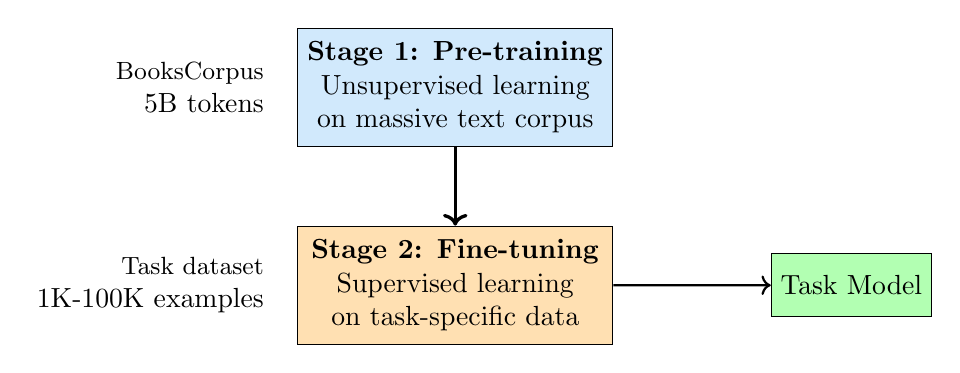
\begin{tikzpicture}[scale=0.85][node distance=2cm]
            % Stage 1
            \node[draw, rectangle, fill=lightblue!30, minimum width=4cm, minimum height=1.5cm, align=center] (pretrain)
                {\textbf{Stage 1: Pre-training} \\ Unsupervised learning \\ on massive text corpus};

            % Stage 2
            \node[draw, rectangle, fill=orange!30, minimum width=4cm, minimum height=1.5cm, align=center, below=of pretrain] (finetune)
                {\textbf{Stage 2: Fine-tuning} \\ Supervised learning \\ on task-specific data};

            % Arrow
            \draw[->, very thick] (pretrain) -- (finetune);

            % Data labels
            \node[left=0.3cm of pretrain, align=right] {\small BooksCorpus \\ 5B tokens};
            \node[left=0.3cm of finetune, align=right] {\small Task dataset \\ 1K-100K examples};

            % Output
            \node[draw, rectangle, fill=green!30, minimum width=2cm, minimum height=0.8cm, right=2cm of finetune] (output)
                {Task Model};
            \draw[->, thick] (finetune) -- (output);
        \end{tikzpicture}
    \end{center}

    \vspace{0.3cm}

    \textbf{Why this works:}
    \begin{itemize}\setlength{\itemsep}{0pt}
        \item Pre-training learns general language understanding
        \item Fine-tuning adapts to specific task format
        \item Much less task data needed!
    \end{itemize}
\end{frame}

\begin{frame}[shrink=10]{Pre-training: Language Modeling 📚}
\small
    \textbf{Objective: Predict next token}

    \vspace{0.3cm}

    \begin{block}{Example Training Sequence}
        \textbf{Text:} "The quick brown fox jumps over the lazy dog"

        \vspace{0.3cm}

        \textbf{Training examples:}
        \begin{itemize}\setlength{\itemsep}{0pt}
            \item "The" → predict "quick"
            \item "The quick" → predict "brown"
            \item "The quick brown" → predict "fox"
            \item "The quick brown fox" → predict "jumps"
            \item ...
        \end{itemize}
    \end{block}

    \vspace{0.3cm}

    \textbf{Self-supervised learning:}
    \begin{itemize}\setlength{\itemsep}{0pt}
        \item No manual labels needed!
        \item Every text provides training signal
        \item Can use web-scale data
        \item Model learns: syntax, semantics, facts, reasoning
    \end{itemize}
\end{frame}

\begin{frame}{Fine-tuning for Downstream Tasks 🎯}
    \textbf{Task Format: Input + Delimiter + Label}

    \vspace{0.3cm}

    \begin{columns}[T]
        \begin{column}{0.48\textwidth}
            \textbf{Text Classification:}

            \small
            \texttt{[START] This movie is amazing! [DELIM] [LABEL]}

            \vspace{0.15cm}
            Model predicts: "Positive"

            \vspace{0.15cm}

            \textbf{Entailment:}

            \small
            \texttt{[START] Premise [DELIM] Hypothesis [DELIM] [LABEL]}

            \vspace{0.15cm}
            Model predicts: "Entailment" / "Contradiction" / "Neutral"
        \end{column}

        \begin{column}{0.48\textwidth}
            \textbf{Question Answering:}

            \small
            \texttt{[START] Context [DELIM] Question [DELIM] [ANSWER]}

            \vspace{0.15cm}
            Model predicts answer span

            \vspace{0.15cm}

            \textbf{Similarity:}

            \small
            \texttt{[START] Text1 [DELIM] Text2 [DELIM] [LABEL]}

            \vspace{0.15cm}
            Model predicts similarity score
        \end{column}
    \end{columns}

    \vspace{0.3cm}

    \begin{alertblock}{Key Insight}
        All tasks can be framed as text completion! 🎯
    \end{alertblock}
\end{frame}

\begin{frame}[shrink=10]{Fine-tuning Implementation Details ⚙️}
    \textbf{What changes during fine-tuning?}

    \vspace{0.3cm}

    \begin{enumerate}\setlength{\itemsep}{0pt}
        \item \textbf{Add task-specific input transformations}
        \begin{itemize}\setlength{\itemsep}{0pt}
            \item Format inputs with delimiters
            \item Add special tokens
        \end{itemize}

        \vspace{0.3cm}

        \item \textbf{Add classification head (optional)}
        \begin{itemize}\setlength{\itemsep}{0pt}
            \item Linear layer for classification
            \item Or use language modeling head
        \end{itemize}

        \vspace{0.3cm}

        \item \textbf{Train with supervised objective}
        \begin{itemize}\setlength{\itemsep}{0pt}
            \item Cross-entropy loss
            \item Much lower learning rate
            \item Few epochs (3-5)
        \end{itemize}
    \end{enumerate}

    \vspace{0.3cm}

    \textbf{Hyperparameters:}
    \begin{itemize}\setlength{\itemsep}{0pt}
        \item Learning rate: 6.25e-5 (much lower than pre-training!)
        \item Batch size: 32
        \item Max epochs: 3
        \item Linear learning rate decay to 0
    \end{itemize}
\end{frame}

\section{GPT Performance and Impact}

\begin{frame}{GPT-1 Results 📊}
    \textbf{Performance on GLUE Benchmark:}

    \vspace{0.3cm}

    \begin{table}
        \small
        \begin{tabular}{lcc}
            \toprule
            \textbf{Task} & \textbf{Previous SOTA} & \textbf{GPT} \\
            \midrule
            Natural Language Inference & 88.0 & \textbf{89.9} \\
            Question Answering & 86.7 & \textbf{88.1} \\
            Semantic Similarity & 85.0 & \textbf{85.8} \\
            Text Classification & 93.0 & \textbf{94.2} \\
            \bottomrule
        \end{tabular}
    \end{table}

    \vspace{0.3cm}

    \begin{alertblock}{Key Findings}
        \begin{itemize}\setlength{\itemsep}{0pt}
            \item GPT achieved SOTA on 9 out of 12 tasks studied
            \item Large improvements on tasks with less training data
            \item Transfer learning works for NLP!
        \end{itemize}
    \end{alertblock}

    \vspace{0.3cm}

    \small
    \textit{Reference: Radford et al. (2018) - "Improving Language Understanding by Generative Pre-Training"}
\end{frame}

\begin{frame}[shrink=10]{Zero-Shot and Few-Shot Learning 🎯}
\small
    \begin{discussion}
        What if we could use the model \textit{without} fine-tuning?
    \end{discussion}

    \vspace{0.3cm}

    \textbf{Definitions:}
    \begin{itemize}\setlength{\itemsep}{0pt}
        \item \textbf{Zero-shot}: No task-specific training examples
        \item \textbf{Few-shot}: A few examples (1-10) as context
        \item \textbf{Fine-tuning}: Full supervised training
    \end{itemize}

    \vspace{0.3cm}

    \textbf{GPT-1 observations:}
    \begin{itemize}\setlength{\itemsep}{0pt}
        \item ✅ Fine-tuning works best
        \item ⚠️ Zero-shot performance is weak
        \item 💡 Model has learned a lot, but needs task formatting
    \end{itemize}

    \vspace{0.3cm}

    \begin{thinkaboutit}
        This limitation motivated GPT-2 and GPT-3: Can we make models that work zero-shot?
    \end{thinkaboutit}
\end{frame}

\begin{frame}[shrink=5]{Visualizing What GPT Learns 🎨}
    \begin{center}
        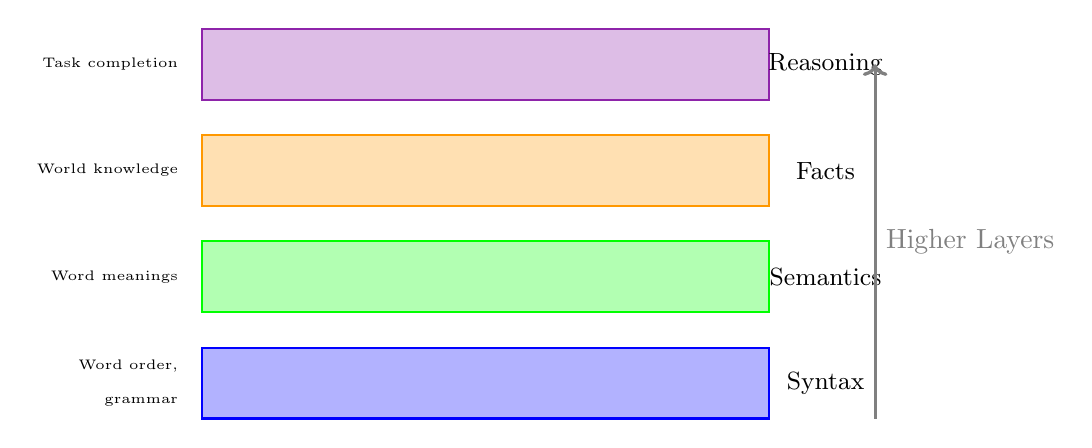
\begin{tikzpicture}[scale=0.9]
            % Layer representations
            \foreach \y/\label/\color in {0/Syntax/blue, 1.5/Semantics/green, 3/Facts/orange, 4.5/Reasoning/purple} {
                \draw[fill=\color!30, draw=\color, thick] (0,\y) rectangle (8,\y+1);
                \node at (8.8,\y+0.5) {\small \label};
            }

            % Gradient arrow
            \draw[->, very thick, gray] (9.5, 0) -- (9.5, 5) node[midway, right] {Higher Layers};

            % Examples
            \node[left, align=right] at (-0.2, 0.5) {\tiny Word order, \\ \tiny grammar};
            \node[left, align=right] at (-0.2, 2) {\tiny Word meanings};
            \node[left, align=right] at (-0.2, 3.5) {\tiny World knowledge};
            \node[left, align=right] at (-0.2, 5) {\tiny Task completion};
        \end{tikzpicture}
    \end{center}

    \vspace{0.3cm}

    \textbf{Layer analysis shows:}
    \begin{itemize}\setlength{\itemsep}{0pt}
        \item Early layers: Syntactic patterns
        \item Middle layers: Semantic understanding
        \item Later layers: Task-specific reasoning
        \item Progressive abstraction!
    \end{itemize}
\end{frame}

\begin{frame}[shrink=10]{The Generative Pre-training Paradigm 🌟}
    \textbf{Why "Generative Pre-Training" was revolutionary:}

    \vspace{0.3cm}

    \begin{enumerate}\setlength{\itemsep}{0pt}
        \item \textbf{Unified Architecture}
        \begin{itemize}\setlength{\itemsep}{0pt}
            \item Same model for all tasks
            \item vs. task-specific architectures
        \end{itemize}

        \vspace{0.3cm}

        \item \textbf{Transfer Learning}
        \begin{itemize}\setlength{\itemsep}{0pt}
            \item Learn once, apply many times
            \item vs. training from scratch
        \end{itemize}

        \vspace{0.3cm}

        \item \textbf{Scalability}
        \begin{itemize}\setlength{\itemsep}{0pt}
            \item More data → Better performance
            \item Clear path to improvement
        \end{itemize}

        \vspace{0.3cm}

        \item \textbf{Simplicity}
        \begin{itemize}\setlength{\itemsep}{0pt}
            \item Just predict next token
            \item No complex objectives
        \end{itemize}
    \end{enumerate}

    \vspace{0.3cm}

    \begin{alertblock}{This paradigm enabled GPT-2, GPT-3, and beyond!}
    \end{alertblock}
\end{frame}

\section{Discussion and Extensions}

\begin{frame}[shrink=10]{Limitations of GPT-1 ⚠️}
\small
    \textbf{What GPT-1 couldn't do well:}

    \vspace{0.3cm}

    \begin{itemize}\setlength{\itemsep}{0pt}
        \item ❌ \textbf{Zero-shot performance}: Needed fine-tuning for each task
        \item ❌ \textbf{Model size}: 117M parameters (small by today's standards)
        \item ❌ \textbf{Training data}: Limited to ~5B tokens
        \item ❌ \textbf{Context length}: Only 512 tokens
        \item ❌ \textbf{Generation quality}: Sometimes incoherent
        \item ❌ \textbf{Factual accuracy}: Prone to hallucinations
    \end{itemize}

    \vspace{0.3cm}

    \begin{discussion}
        How would you address these limitations? \\
        \vspace{0.2cm}
        \textit{(Spoiler: GPT-2 and GPT-3 tried to solve these!)}
    \end{discussion}
\end{frame}

\begin{frame}{Comparison with BERT 🔄}
    \begin{table}
        \small
        \begin{tabular}{lcc}
            \toprule
            \textbf{Aspect} & \textbf{BERT} & \textbf{GPT} \\
            \midrule
            Architecture & Encoder only & Decoder only \\
            Training objective & Masked LM & Autoregressive LM \\
            Context & Bidirectional & Left-to-right \\
            Best for & Understanding & Generation \\
            Fine-tuning & Task-specific heads & Unified format \\
            Parameters (base) & 110M & 117M \\
            \bottomrule
        \end{tabular}
    \end{table}

    \vspace{0.3cm}

    \begin{thinkaboutit}
        BERT dominated understanding tasks (2018-2019), but GPT's approach proved more scalable and versatile. Why?
    \end{thinkaboutit}

    \vspace{0.3cm}

    \textbf{Answer:} Autoregressive modeling naturally supports generation, which unlocks zero-shot and few-shot capabilities!
\end{frame}

\begin{frame}[shrink=10]{Key Takeaways 🔑}
    \begin{enumerate}\setlength{\itemsep}{0pt}
        \item \textbf{GPT introduced generative pre-training}
        \begin{itemize}\setlength{\itemsep}{0pt}
            \item Transformer decoder architecture
            \item Autoregressive language modeling
        \end{itemize}

        \vspace{0.3cm}

        \item \textbf{Two-stage training paradigm}
        \begin{itemize}\setlength{\itemsep}{0pt}
            \item Unsupervised pre-training on massive text
            \item Supervised fine-tuning on task data
        \end{itemize}

        \vspace{0.3cm}

        \item \textbf{Masked self-attention is key}
        \begin{itemize}\setlength{\itemsep}{0pt}
            \item Enables autoregressive generation
            \item Prevents information leakage
        \end{itemize}

        \vspace{0.3cm}

        \item \textbf{Transfer learning for NLP}
        \begin{itemize}\setlength{\itemsep}{0pt}
            \item Learn general patterns once
            \item Apply to many tasks
        \end{itemize}

        \vspace{0.3cm}

        \item \textbf{Foundation for modern LLMs}
        \begin{itemize}\setlength{\itemsep}{0pt}
            \item GPT-2, GPT-3, ChatGPT all build on this
        \end{itemize}
    \end{enumerate}
\end{frame}

\begin{frame}{Readings 📖}
    \begin{block}{Required Reading}
        \textbf{Radford et al. (2018)} - "Improving Language Understanding by Generative Pre-Training" \\
        \href{https://cdn.openai.com/research-covers/language-unsupervised/language_understanding_paper.pdf}{[PDF]}
    \end{block}

    \vspace{0.3cm}

    \begin{block}{Recommended Readings}
        \begin{itemize}\setlength{\itemsep}{0pt}
            \item \textbf{Vaswani et al. (2017)} - "Attention is All You Need" \\
            \href{https://arxiv.org/abs/1706.03762}{[ArXiv]}

            \item \textbf{Devlin et al. (2018)} - "BERT: Pre-training of Deep Bidirectional Transformers" \\
            \href{https://arxiv.org/abs/1810.04805}{[ArXiv]}

            \item \textbf{The Illustrated GPT-2} by Jay Alammar \\
            \href{https://jalammar.github.io/illustrated-gpt2/}{[Blog]}
        \end{itemize}
    \end{block}
\end{frame}

\begin{frame}{Next Lecture Preview 🔮}
\small
    \begin{block}{Lecture 19: Scaling Up to GPT-3 and Beyond}
        \begin{itemize}\setlength{\itemsep}{0pt}
            \item GPT-2: Language models as unsupervised multitask learners
            \item GPT-3: Few-shot learning at scale
            \item Scaling laws: Why bigger is better
            \item Emergent abilities of large language models
            \item From GPT-3 to ChatGPT
        \end{itemize}
    \end{block}

    \vspace{0.5cm}

    \begin{center}
        \Large{Questions? 💬}
    \end{center}
\end{frame}

\end{document}
